%
% ringe.tex -- Grundlegende Konstruktionen für Ringe
%
% (c) 2021 Prof Dr Andreas Müller, OST Ostschweizer Fachhochschule
%
\subsection{Ringe und Moduln
\label{buch:grundlagen:subsection:ringe}}
Die ganzen Zahlen haben ausser der Addition mit neutralem Element $0$
auch noch eine Multiplikation mit dem neutralen Element $1$.
Die Multiplikation ist aber nicht immer invertierbar und zwar
nicht nur für $0$.
Eine ähnliche Situation haben wir bei $M_n(\Bbbk)$ angetroffen.
$M_n(\Bbbk)$ ist eine zunächst eine Gruppe bezüglich der Addition,
hat aber auch noch eine Multiplikation, die nicht immer umkehrbar ist.
Diese Art von Struktur nennt man einen Ring.

\subsubsection{Definition eines Rings}

\begin{definition}
\index{Ring}%
Eine Menge $R$ mit einer additiven Operation $+$ mit neutralem Element
$0$ und einer multiplikativ geschriebenen Operation $\cdot$ heisst ein
{\em Ring}, wenn folgendes gilt.
\begin{enumerate}
\item
$R$ ist eine Gruppe bezüglich der Addition.
\item
$R\setminus\{0\}$ ist eine Halbgruppe.
\item
Es gelten die {\em Distributivgesetze}
\[
a(b+c)=ab+ac
\qquad\text{und}\qquad
(a+b)c=ac+bc
\]
für beliebige Elemente $a,b,c\in R$.
\index{Distributivgesetz}%
\end{enumerate}
\end{definition}

Die Distributivgesetze stellen sicher, dass man in $R$ beliebig
ausmultiplizieren kann.
Man kann also so rechnen kann, wie man sich das gewohnt ist.
Es stellt auch sicher, dass die Multiplikation mit $0$ immer $0$
ergibt, denn es ist
\[
r0 = r(a-a) = ra-ra=0.
\]

Man beachte, dass weder verlangt wurde, dass die Multiplikation
ein neutrales Element hat oder kommutativ ist.
Der Ring $\mathbb{Z}$ erfüllt beide Bedingungen.
Die Beispiele weiter unten werden zeigen, dass es auch Ringe gibt,
in denen die Multiplikation nicht kommutativ ist, die Multiplikation
kein neutrales Element hat oder beides.

\begin{definition}
\index{Ring mit Eins}%
Ein Ring $R$ heisst ein Ring mit Eins, wenn die Multiplikation ein
neutrales Element hat.
\end{definition}

\begin{definition}
\index{Ring!kommutativ}%
\index{kommutativer Ring}%
Ein Ring $R$ heisst kommutativ, wenn die Multiplikation kommutativ
ist.
\end{definition}

\subsubsection{Beispiele von Ringen}

\begin{beispiel}
Alle Zahlenkörper aus Kapitel~\ref{buch:chapter:zahlen} sind kommutative
Ringe mit Eins.
\end{beispiel}

\begin{beispiel}
Die Menge $c(\mathbb{Z})$ der Folgen $(a_n)_{n\in\mathbb{N}}$ mit
Folgengliedern in $\mathbb{Z}$ wird eine Ring, wenn man die Addition
und Multiplikation elementweise definiert, also
\begin{align*}
&\text{Addition:}
&
a+b&\text{\;ist die Folge mit Folgengliedern}&
(a+b)_n &= a_nb_n \quad\text{für alle $n\in\mathbb{N}$}
\\
&\text{Multiplikation:}
&
a\cdot b&\text{\;ist die Folge mit Folgengliedern}&
(a\cdot b)_n &=  a_nb_n \quad\text{für alle $n\in\mathbb{N}$}
\end{align*}
für $a,b\in c(\mathbb{Z})$.
Die Algebra ist kommutativ und hat die konstante Folge 
$u_n = 1\;\forall n$ als Eins.

Wir betrachten jetzt ein Unterring $c_0(\mathbb{Z})\subset c(\mathbb{Z})$
bestehend aus den Folgen, die nur für endlich viele Folgenglieder von
$0$ verschieden sind.
Für eine Folge $a\in c_0(\mathbb{Z})$ gibt es eine Zahl $N$ derart, dass
$a_n=0$ für $n\ge N$.
Die konstante Folge $u_n=1$, die in $c(\mathbb{Z})$ erfüllt diese
Bedingung nicht, die Eins des Ringes $c(\mathbb{Z})$ ist also nicht in
$c_0(\mathbb{Z})$.
$c_0(\mathbb{Z})$ ist immer noch ein Ring, aber er hat kein Eins.
\end{beispiel}

\begin{beispiel}
\begin{figure}
\centering
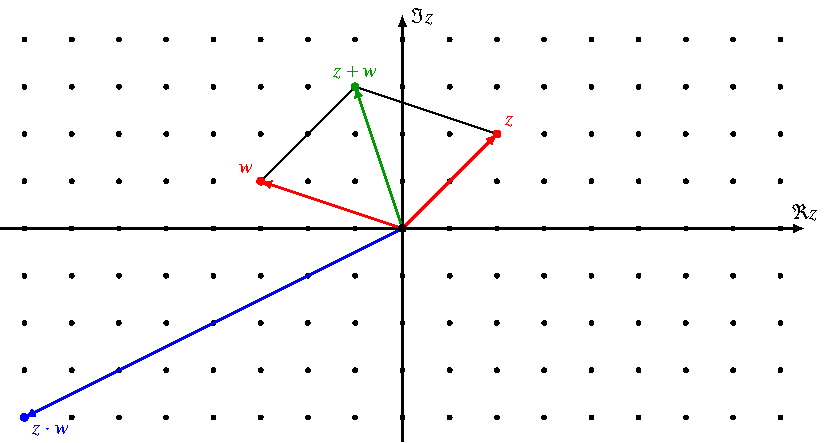
\includegraphics{chapters/10-vektorenmatrizen/images/gausszahlen.pdf}
\caption{Der Ring der ganzen Gausschen Zahlen besteht aus den ganzahligen
Gitterpunkten in der Gausschen Zahlenebene
\label{buch:vektorenmatrizen:fig:ganzgauss}}
\end{figure}
Die Menge
\[
\mathbb{Z} + i\mathbb{Z}
=
\{a+bi\;|\; a,b\in\mathbb{Z}\}
=
\mathbb{Z}[i]
\subset
\mathbb{C}
\]
ist eine Teilmenge von $\mathbb{C}$ und erbt natürlich die 
arithmetischen Operationen.
Die Summe zweier solcher Zahlen $a+bi\in\mathbb{Z}[i]$ und
$c+di\in\mathbb{Z}[i]$ ist
$(a+bi)+(c+di)=(a+c) + (b+d)i\in \mathbb{Z}[i]$, weil $a+c\in\mathbb{Z}$
und $b+d\in\mathbb{Z}$ ganze Zahlen sind.
Ebenso ist das Produkt dieser Zahlen
\(
(a+bi)(c+di)
=
(ac-bd) + (ad+bc)i
\in \mathbb{Z}[i]
\)
weil Realteil $ac-bd\in\mathbb{Z}$ und der Imaginärteil $ad+bc\in\mathbb{Z}$
ganze Zahlen sind.
Die Menge $\mathbb{Z}[i]$ ist also ein kommutative Ring mit Eins, er
heisst der Ring der ganzen {\em Gaussschen Zahlen}.
\index{Gausssche Zahlen}%
\end{beispiel}

\begin{beispiel}
Die Menge der Matrizen $M_n(\mathbb{Z})$ ist ein Ring mit Eins.
Für $n>1$ ist er nicht kommutativ.
Der Ring $M_2(\mathbb{Z})$ enthält den Teilring
\[
G
=
\biggl\{
\begin{pmatrix}
a&-b\\b&a
\end{pmatrix}
\;\bigg|\;
a,b\in\mathbb{Z}
\biggr\}
=
\mathbb{Z}+ \mathbb{Z}J
\subset
M_2(\mathbb{Z}).
\]
Da die Matrix $J$ die Relation $J^2=-E$ erfüllt, ist der Ring $G$
nichts anderes als der Ring der ganzen Gaussschen Zahlen.
Der Ring $\mathbb{Z}[i]$ ist also ein Unterring des Matrizenrings
$M_2(\mathbb{Z})$.
\end{beispiel}

\subsubsection{Einheiten}
In einem Ring mit Eins sind normalerweise nicht alle von $0$ verschiedenen
Elemente intertierbar.
Die Menge der von $0$ verschiedenen Elemente in $R$ wir mit $R^*$
bezeichnet.
\index{$R^*$}%
Die Menge der invertierbaren Elemente verdient einen besonderen Namen.

\begin{definition}
Ist $R$ ein Ring mit Eins, dann heissen die Elemente von
\[
U(R) = \{ r\in R \;|\; \text{$r$ in $R$ invertierbar}\}.
\]
die {\em Einheiten} von $R$.
\index{Einheit}%
\end{definition}

\begin{satz}
$U(R)$ ist eine Gruppe, die sogenannte {\em Einheitengruppe}.
\index{Einheitengruppe}%
\end{satz}

\begin{beispiel}
Die Menge $M_2(\mathbb{Z})$ ist ein Ring mit Eins, die Einheitengruppe
besteht aus den invertierbaren $2\times 2$-Matrizen. 
Aus der Formel für 
\[
\begin{pmatrix}
a&b\\
c&d
\end{pmatrix}^{-1}
=
\frac{1}{ad-bc}\begin{pmatrix}
d&-b\\
-c&a
\end{pmatrix}
\]
zeigt, dass $U(M_2(\mathbb{Z})) = \operatorname{SL}_2(\mathbb{Z})$.
\end{beispiel}

\begin{beispiel}
Die Einheitengruppe von $M_n(\Bbbk)$ ist die allgemeine lineare Gruppe 
$U(M_n(\Bbbk))=\operatorname{GL}_n(\Bbbk)$.
\end{beispiel}

\subsubsection{Nullteiler}
Ein möglicher Grund, warum ein Element $r\in R$ nicht invertierbar
ist, kann sein, dass es ein Element $s\in R$ gibt mit $rs=0$.
Wäre nämlich $t$ ein inverses Element, dann wäre $0=t0 = t(rs) = (tr)s=s$.

\begin{definition}
Ein Element $r\in R^*$ heisst ein {\em Nullteiler} in $R$,
wenn es ein $s\in R^*$ gibt mit $rs=0$
Ein Ring ohne Nullteiler heisst {\em nullteilerfrei}.
\end{definition}

In $\mathbb{R}$ ist man sich gewohnt zu argumentieren, dass wenn ein
Produkt $ab=0$ ist, dann muss einer der Faktoren $a=0$ oder $b=0$ sein.
Dieses Argument funktioniert nur, weil $\mathbb{R}$ ein nullteilerfreier
Ring ist.
In $M_2(\mathbb{R})$ ist dies nicht mehr möglich.
Die beiden Matrizen
\[
A=\begin{pmatrix}
1&0\\0&0
\end{pmatrix}
,\qquad
B=\begin{pmatrix}
0&0\\0&1
\end{pmatrix}
\qquad\Rightarrow\qquad
AB=0
\]
sind Nullteiler in $M_2(\mathbb{Z})$.

\subsubsection{Homomorphismus}
Eine Abbildung zwischen Ringen muss die algebraische Struktur respektieren,
wenn sich damit Eigenschaften vom einen Ring auf den anderen transportieren
lassen sollen.

\begin{definition}
Eine Abbildung $\varphi:R \to S$ zwischen Ringen heisst ein
{\em Homomorphismus}
\index{Homomorphismus}%
oder {\em Ringhomomorphismus},
\index{Ringhomomorphismus}%
wenn $\varphi$ ein Gruppenhomomorphismus der additiven Gruppen der Ringe
ist und ausserdem gilt
\[
\varphi(r_1r_2) = \varphi(r_1)\varphi(r_2).
\]
Der Kern ist die Menge
\[
\ker\varphi = \{ r\in R\;|\; \varphi(r)=0\}
\]
\index{Kern}%
\end{definition}

Wieder hat der Kern zusätzliche Eigenschaften.
Er ist natürlich bezüglich der additiven Struktur des Ringes ein
Normalteiler, aber weil die additive Gruppe ja abelsch ist, ist das
keine wirkliche Einschränkung.
Für ein beliebiges Element $r\in R$ und $k\in \ker\varphi$ gilt
\begin{align*}
\varphi(kr) &= \varphi(k)\varphi(r) = 0\cdot\varphi(r) = 0
\\
\varphi(rk) &= \varphi(r)\varphi(k) = \varphi(r)\cdot 0 = 0.
\end{align*}
Für den Kern gilt also, dass $\ker\varphi\cdot R\subset \ker\varphi$
und $R\cdot\ker\varphi\subset\ker\varphi$.

\subsubsection{Ideale}
\begin{figure}
\centering
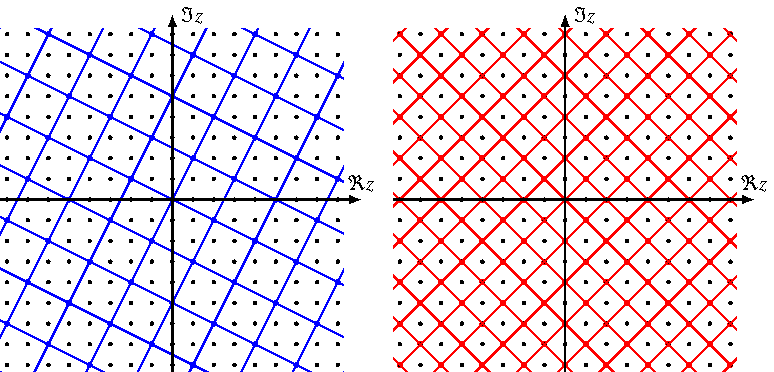
\includegraphics{chapters/10-vektorenmatrizen/images/ideale.pdf}
\caption{Ideale im Ring der ganzen Gaussschen Zahlen $\mathbb{Z}[i]$.
Für jedes Element $r\in \mathbb{Z}[i]$ ist die Menge  $r\mathbb{Z}[i]$
ein ein Ideal in $\mathbb{Z}[i]$.
Links das Ideal $(1+2i)\mathbb{Z}[i]$ (blau), rechts das Ideal
$(1+i)\mathbb{Z}[i]$ (rot).
\label{buch:vektorenmatrizen:fig:ideale}}
\end{figure}
Bei der Betrachtung der additiven Gruppe des Ringes $\mathbb{Z}$ der
ganzen Zahlen wurde bereits die Untergruppe $n\mathbb{Z}$ diskutiert
und die Faktorgruppe $\mathbb{Z}/n\mathbb{Z}$ der Reste konstruiert.
Reste können aber auch multipliziert werden, es muss also auch möglich
sein, der Faktorgruppe eine multiplikative Struktur zu verpassen.

Sei jetzt also $I\subset R$ ein Unterring.
Die Faktorgruppe $R/I$ hat bereits die additive Struktur, es muss
aber auch die Multiplikation definiert werden.
Die Elemente $r_1+I$ und $r_2+I$ der Faktorgruppe $R/I$ haben das
Produkt
\[
(r_1+I)(r_2+I)
=
r_1r_2 + r_1I + Ir_2 + II.
\]
Dies stimmt nur dann mit $r_1r_2+I$ überein, wenn $r_1I\subset I$ und
$r_2I\subset I$ ist.

\begin{definition}
Ein Unterring $I\subset R$ heisst ein {\em Ideal}, wenn für jedes $r\in R$ gilt
$rI\subset I$ und $Ir\subset I$ gilt.
\index{Ideal}%
Die Faktorgruppe $R/I$ erhält eine natürliche Ringstruktur, $R/I$ 
heisst der {\em Quotientenring}.
\index{Quotientenring}%
\end{definition}

\begin{beispiel}
Die Menge $n\mathbb{Z}\subset\mathbb{Z}$ besteht aus den durch $n$ teilbaren
Zahlen.
Multipliziert man durch $n$ teilbare Zahlen mit einer ganzen Zahl,
bleiben sie durch $n$ teilbar, $n\mathbb{Z}$ ist also ein Ideal in
$\mathbb{Z}$.
Der Quotientenring ist der Ring der Reste bei Teilung durch $n$,
er wird in 
Kapitel~\ref{buch:chapter:endliche-koerper}
im Detail untersucht.
\end{beispiel}

Ein Ideal $I\subset R$ drückt als die Idee ``gemeinsamer Faktoren''
auf algebraische Weise aus und der Quotientenring $R/I$ beschreibt
das, was übrig bleibt, wenn man diese Faktoren ignoriert.

\begin{beispiel}
In Abbildung~\ref{buch:vektorenmatrizen:fig:ideale} sind zwei
Ideale im Ring der ganzen Gaussschen Zahlen dargestellt.
Die blauen Punkte sind $I_1=(1+2i)\mathbb{Z}$ und die roten Punkte sind
$I_2=(1+i)\mathbb{Z}$.
Die Faktorgruppen $R/I_1$ und $R/I_2$ fassen jeweils Punkte, die sich
um ein Element von $I_1$ bzw.~$I_2$ unterscheiden, zusammen.

Im Falle von $I_2$ gibt es nur zwei Arten von Punkten, nämlich
die roten und die schwarzen, der Quotientenring hat
daher nur zwei Elemente, $R/I_2 = \{0+I_2,1+I_2\}$.
Wegen $1+1=0$ in diesem Quotientenring, ist $R/I_2=\mathbb{Z}/2\mathbb{Z}$.

Im Falle von $I_1$ gibt es fünf verschiedene Punkte, als Menge ist
\[
R/I_1 
=
\{
0+I_1,
1+I_1,
2+I_1,
3+I_1,
4+I_1
\}.
\]
Die Rechenregeln sind also dieselben wie im Ring $\mathbb{Z}/5\mathbb{Z}$.
In gewisser Weise verhält sich die Zahl $1+2i$ in den ganzen 
Gaussschen Zahlen bezüglich Teilbarkeit ähnlich wie die Zahl $5$ in den
ganzen Zahlen.
\end{beispiel}

